\titre{3 étapes :}
\begin{enumerate}
	\item Diviser le problème initial en plusieurs sous problèmes.
	\item Régner : Si la taille d'un sous problème est assez petite, on le résoud. Sinon récursion.
	\item Combiner : On forme la solution au problème initial en combinant les solutions aux sous problèmes.
\end{enumerate}

\titre{Schéma : }\\
Fonction DPR(Probleme P)\\
Debut\\
	\hspace*{1cm} Si taille(P) petite alors Resoudre(P)\\
	\hspace*{1cm} Sinon \\
		\hspace*{2cm} Diviser P en P$_1$, P$_2$, \ldots, P$_k$ \\
		\hspace*{2cm} Pour i de 1 à $k$ S$_i$ = DPR(P$_i$) FinPour \\
		\hspace*{2cm} Combiner(S$_1$,\ldots,S$_n$)\\
Fin\\

\titre{Théorème Maître:} 
\begin{itemize}
	\item Si $f(n) = O(n^{\mathrm{log}_ba-\varepsilon})$ ($\varepsilon > 0)$ alors $T(n)\in O(n^{\mathrm{log}_ba})$
	\item Si $f(n) = \theta(n^{\mathrm{log}_ba})$ alors $T(n) = O(n^{\mathrm{log}_ba}\ln n)$
	\item Si $f(n) = \Omega(n^{\mathrm{log}_ba+\varepsilon})$ ($\varepsilon > 0$). Alors $T(n) \in O(f(n))$
\end{itemize}

\newpage

\titre{Représentation des appels récursifs par un arbre :}\\

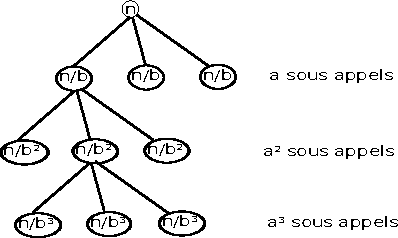
\includegraphics[width=250px]{Images/03_arbreDR.pdf}\\

\begin{tabular}{l|l|l|}
Niveau & Nb Noeuds & Temps pour ce niveau \\ \hline
0 & 1 & $f(n)$ \\ \hline
1 & $a$ & $af(\frac{n}{b})$ \\ \hline
2 & $a^2$ & $a^2f(\frac{n}{b^2})$ \\ \hline
3 & $a^3$ & $a^3f(\frac{n}{b^3})$ \\ \hline
\vdots & \vdots & \vdots 
\end{tabular}
\\
\begin{enumerate}
	\item hauteur de l'arbre : $\frac{n}{b^h} = 1 \equiv h = \log_bn$
	\item Nb de noeuds dans l'arbre : $a^0+a^1+a^2+\ldots+a^h = \frac{1+a^{h+1}}{1-a} = C + C2a^h$. Or $a^h = a^{\log_bn}=(b^{\log_ba})^{\log_bn} =  (b^{\log_bn})^{\log_ba} = n^{\log_ba}$. Donc le nombre de noeuds dans l'arbre est en $O(n^{\log_ba})$.
	\item La complexité de l'algorithme dépend ce qui compte le plus de $f(n)$ ou du nombre de noeuds dans l'arbre. Il y a donc trois cas.
\end{enumerate}



